

\begin{frame}
  \frametitle{Test convergence in cluster size}
  \begin{tabular}[h]{cc}
    \begin{minipage}[h]{0.55\linewidth}
      \begin{center}
        %Below the plasmon resonance ($\sim40\,\mathrm{eV}$), 
        At low energy,%
        the photoelectron mean free path is quite large and it
        probes a large cluster of atoms.
        \begin{block}{The big question}
          How many atoms must be included in the cluster for a good
          \textsc{feff} calculation?
        \end{block}
        \begin{block}{The general answer}
          \centering{\color{red}Who knows?}
        \end{block}
        {\pto} has $c>a$ and the O and Ti atoms are displaced from
        sites of centrosymmetry.
      \end{center}
    \end{minipage} &
    \begin{minipage}[h]{0.43\linewidth}
      \begin{center}
        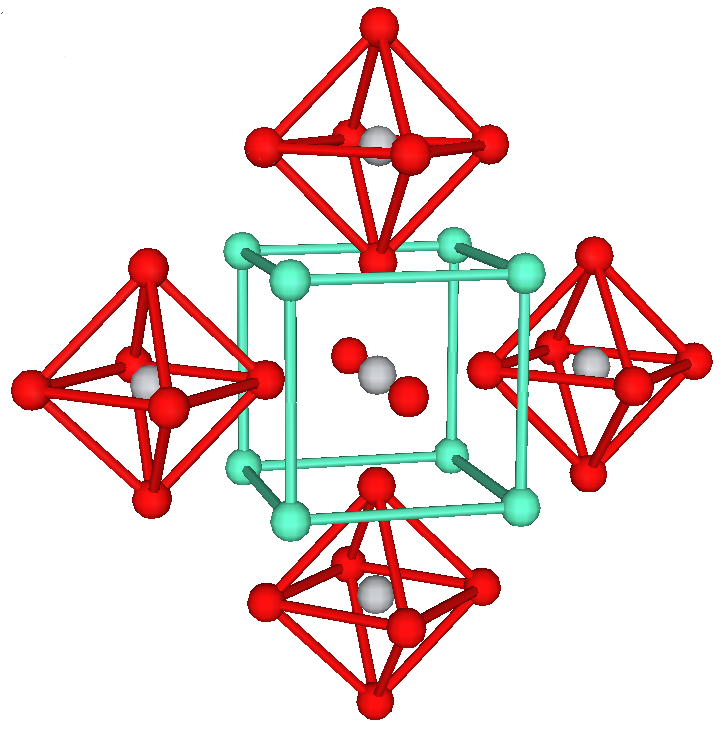
\includegraphics[height=0.95\linewidth]{images/PbTiO3/perovskite}

        \bigskip

        {\pto}: a tetragonally distorted perovskite\\
        {\color{SeaGreen2}$\bullet$} = Pb\quad
        {\color{Gray0}$\bullet$} = Ti\quad
        {\color{Red2}$\bullet$} = O
      \end{center}
    \end{minipage} \\
  \end{tabular}

\end{frame}

\begin{frame}
  \frametitle<1>{First coordination shell of \pto}
  \frametitle<2>{Second coordination shell of \pto}
  \frametitle<3>{Third coordination shell of \pto}
  \frametitle<4>{Fourth coordination shell of \pto}
  \frametitle<5>{Fifth coordination shell of \pto}
  \frametitle<6>{Sixth coordination shell of \pto}

  \setbeamercovered{transparent={50}}
  \begin{columns}[c]
    \begin{column}[c]{0.48\linewidth}
      \includegraphics<1>[width=0.85\linewidth]{images/PbTiO3/shell1}
      \includegraphics<2>[width=0.85\linewidth]{images/PbTiO3/shell2}
      \includegraphics<3>[width=0.85\linewidth]{images/PbTiO3/shell3}
      \includegraphics<4>[width=0.85\linewidth]{images/PbTiO3/shell4}
      \includegraphics<5>[width=0.85\linewidth]{images/PbTiO3/shell5}
      \includegraphics<6>[width=0.85\linewidth]{images/PbTiO3/shell6}
    \end{column}
    \begin{column}[c]{0.48\linewidth}
      \begin{enumerate}
      \item<1-| alert@1> \texttt{O:~~~}R=2.40\AA, 7 atoms
      \item<2-| alert@2| uncover@2-> \texttt{Pb:~~}R=3.60\AA, 15 atoms
      \item<3-| alert@3| uncover@3-> \texttt{Ti:~~}R=4.20\AA, 21 atoms
      \item<4-| alert@4| uncover@4-> \texttt{O:~~~}R=5.00\AA, 45 atoms
      \item<5-| alert@5| uncover@5-> \texttt{Ti:~~}R=5.71\AA, 57 atoms
      \item<6-| alert@6| uncover@6-> \texttt{O:~~~}R=6.30\AA, 86 atoms
      \end{enumerate}
    \end{column}
  \end{columns}

  \bigskip

  \begin{block}{Comment}
    \begin{minipage}[h][10ex][t]{1.0\linewidth}
      \only<1>{We see some indication of the structure just above the
        Fermi energy, but not much else.  Note that the memory
        requirement of the calculation goes as the square of the matrix
        size and the time goes as its cube!}%%
      \only<2>{The XANES structure begins to take shape, but all the
        features are broad.}%%
      \only<3>{Very little changes by adding the 3$^{\mathrm{rd}}$ shell
        Ti atoms!}%%
      \only<4>{Adding an oxygen shell causes the features to become much
        more distinct. Low Z elements have strong scattering at low k.
        High Z elements have strong scattering at high k.}%%
      \only<5>{Again, adding a metal shell does little for the
        spectrum.}%%
      \only<6>{Once again, adding an oxygen shell causes the features to
        become much more distinct. Low Z elements have a strong effect
        on the XANES.  Is the calculation converged?  Probably not.
        Large clusters are required!}%%
    \end{minipage}
  \end{block}
\end{frame}

\begin{frame}
  \frametitle{Scattering amplitude as a function of Z}
  PbTiO$_3$ has three very different elements:
  \begin{description}[Transition metal]
  \item[Low Z] Large at low $k$, tails off quickly
  \item[Transition metal] Large at intermediate $k$, tails off slowly
  \item[Heavy metal] Always there, but with a Ramsauer-Townsend minimum
  \end{description}

  \medskip

  \begin{columns}
    \begin{column}{0.6\linewidth}
      \centering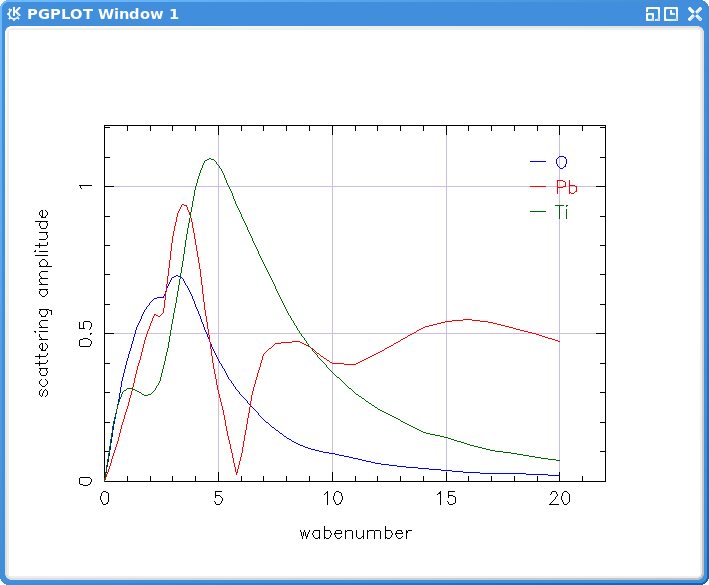
\includegraphics[width=0.85\linewidth]{images/PbTiO3/fofk}
    \end{column}
    %%
    \begin{column}{0.4\linewidth}
      \begin{block}{XANES and EXAFS}
        We can understand both the behavior of the XANES calculations
        and what we observe in EXAFS data.
    \end{block}
    \end{column}
  \end{columns}
\end{frame}

\begin{frame}
  \frametitle{Linear dichroism in \pto}
  \begin{columns}
    \begin{column}{0.48\linewidth}
      \begin{block}{$\overline{ab}$ plane}
        \centering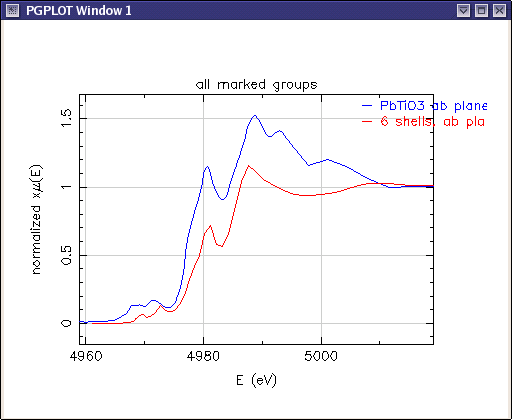
\includegraphics[width=0.85\linewidth]{images/PbTiO3/ab}
      \end{block}
    \end{column}
    \begin{column}{0.48\linewidth}
      \begin{block}{$\hat{c}$ axis}
        \centering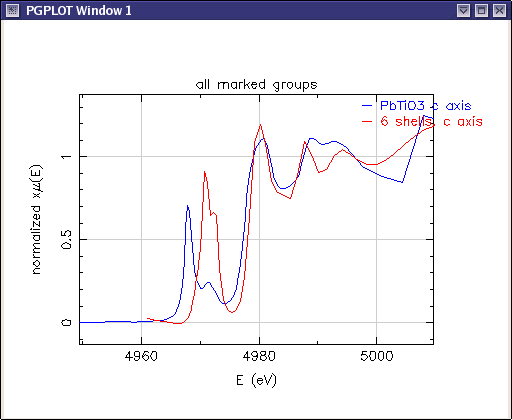
\includegraphics[width=0.85\linewidth]{images/PbTiO3/c}
      \end{block}
    \end{column}
  \end{columns}

  \bigskip

  \begin{center}
    Polarization can be included directly in the XANES calculation and
    shows the correct behavior compared to the data.
  \end{center}
\end{frame}

%%% Local Variables:
%%% mode: latex
%%% TeX-master: t
%%% End:
